\chapter{Supplemental for Chapter \refchB}
%\counterwithin{figure}{section}
%\beginsupplement


\begin{figure}[H]
\centering
    % /Users/janet/Dropbox/meta4_bins_data_and_files/170124_current_metabat_analysis_figures/170124_bad_low_o2_samples_have_more_reads_on_short_contigs--binning_not_considered.pdf
    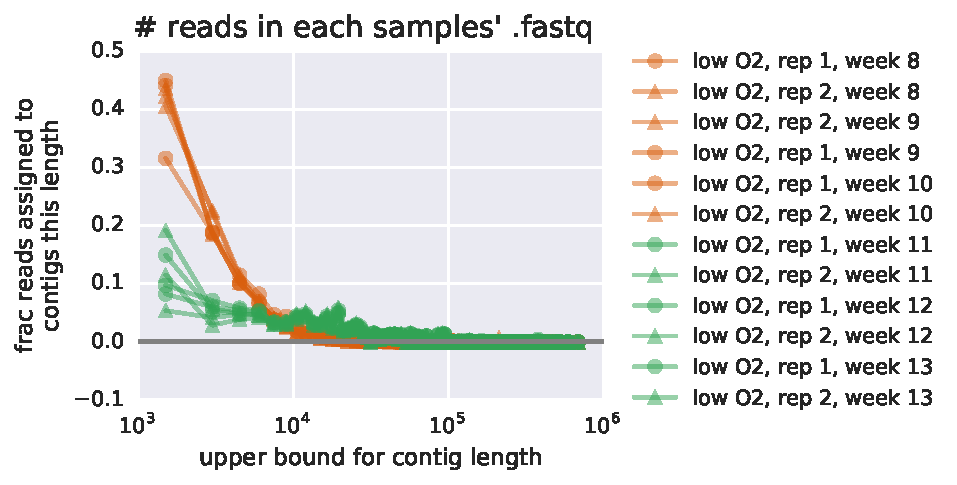
\includegraphics[width=1.0\textwidth]{./tex/chapter2/figures/170124_bad_low_o2_samples_have_more_reads_on_short_contigs--binning_not_considered.pdf}
    \begin{singlespace}
    \caption[Samples best explained by bins have more reads drawn to longer contigs]{
        Samples with metagenomes that are well represented by MetaBAT bins have more reads drawn to longer contigs.}
    \label{fig:contig_dist}
    \end{singlespace}
\end{figure}

\begin{figure}[H]
\centering
    %
    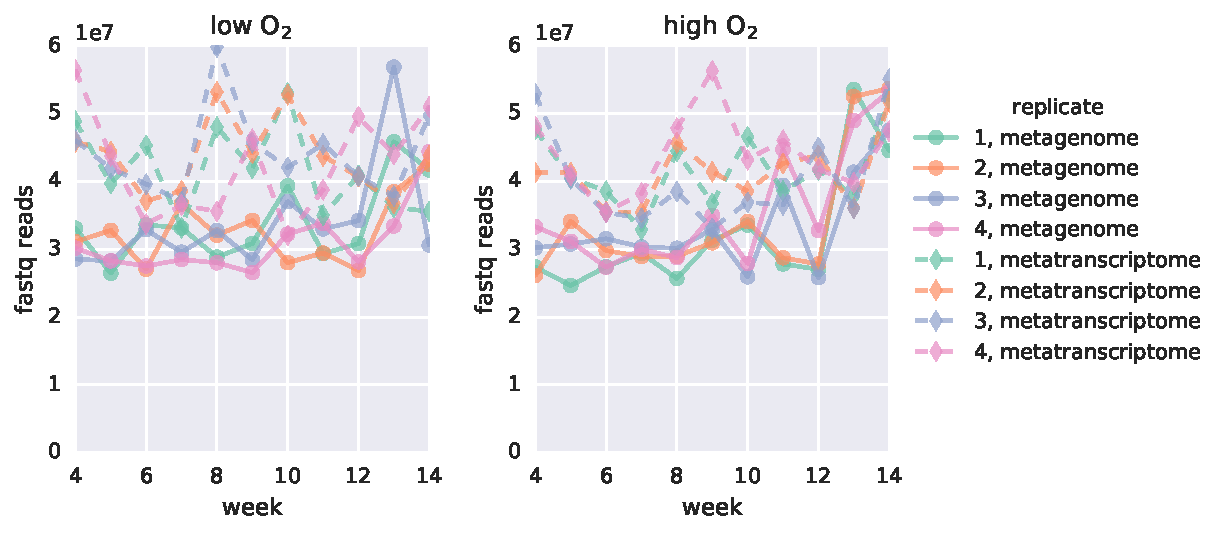
\includegraphics[width=1.0\textwidth]{./tex/chapter2/figures/170326_compare_raw_fastq_reads.pdf}
    \begin{singlespace}
    \caption[Number of reads in metagenomes and metatranscriptomes, by sample]{
        Number of reads in metagenomes and metatranscriptomes, by sample.}
    \label{fig:fastq_reads}
    \end{singlespace}
\end{figure}

